%%%%%%%%%%%%%%%%%%%%%%%%%%%%%%%%%%%%%%%%%%%%%%%%%%%%%%%%%%%%%%%%%%%%%%%%%%%%%%%
%%  sec_b_results_mech.tex --- Results sections B: certification, mechanism,
%%  real-lens.  \input into main.tex; assumes the shared preamble of the
%%  previous campaign's report (tech-report.sty + macros \gammaEPL, \thetaE,
%%  \Rhat, \ESS, \eop, \foundry, \gigalens, \gigalenstwo, \dfile, \art).
%%
%%  Every number in this file is traced to an on-disk artifact per
%%  research/synthesis_tables.md (the spine); its DISCREPANCY FLAGS are
%%  binding and the ARTIFACT value is quoted throughout.  Honest negatives
%%  are first-class results with their own subsection headers (house style).
%%  Scene-substrate results carry the "UNCERTIFIED --- external" label:
%%  "validated" is reserved for the certified old stack; results produced on
%%  the upstream development branch's scene API are proposed to the upstream
%%  team as measurements, with certification theirs to grant
%%  (papers/handoff/CLAIMS.md).
%%%%%%%%%%%%%%%%%%%%%%%%%%%%%%%%%%%%%%%%%%%%%%%%%%%%%%%%%%%%%%%%%%%%%%%%%%%%%%%

%%%%%%%%%%%%%%%%%%%%%%%%%%%%%%%%%%%%%%%%%%%%%%%%%%%%%%%%%%%%%%%%%%%%%%%%%%%%%%%
\section{Results I --- Certification: the Scene API Reproduces the
         Validated Stack}
\label{sec:cert}
%%%%%%%%%%%%%%%%%%%%%%%%%%%%%%%%%%%%%%%%%%%%%%%%%%%%%%%%%%%%%%%%%%%%%%%%%%%%%%%

\noindent\emph{The campaign's foundation result: the next-generation scene
API --- the team's upstream development branch, vendored unpatched at commit
\dfile{80916d2} --- evaluates the same forward model, likelihood, and
gradients as the previous campaign's validated stack to within machine
precision, on both campaign machines, for the configuration class of the real
lens. Everything downstream (the mechanism program of
\S\ref{sec:mech}, the cross-stack reproduction of \S\ref{sec:l0g2}) stands on
this section. All scene-substrate numbers are proposed
(UNCERTIFIED---external): we are the producer; the upstream team is the
grader.}

\medskip
The certification battery F1--F8 compares the scene API's simulator and
likelihood surfaces against the
validated \dfile{58ec9a7} stack of the preceding campaign on the same
\foundry\ inputs (\dfile{v2d} native and \dfile{v3b} binned products), at the
reference point plus three seeded perturbations, compared in constrained
parameter space. The battery ran at zero A100 cost (phoenix L4 free tier);
its Perlmutter repetition (F8) took 58~s of A100 time.

\subsection{The F1--F8 parity battery, both machines}
\label{sec:parity}

All hard gates pass on both machines
(Table~\ref{tab:parity}).\art{data/parity\_report\_scene.json;
data/results-perlmutter/\allowbreak
parity\_report\_scene\_pmnative\_55980038.json} The
forward image and design columns agree at the $10^{-15}$ level --- the two
stacks are evaluating the \emph{same function}, not merely similar ones ---
and the constrained-space gradient, which compounds every convention in the
chain (profiles, grids, PSF, masking, bijectors), agrees to
$1.5\times10^{-11}$ relative $L_2$. The Perlmutter-native re-run under the
production pinned environment (jax~0.6.2, x86 A100; job 55980038) passes
every hard gate with the F1 statistic \emph{bit-consistent} with the phoenix
value ($5.682\times10^{-15}$), certifying the stack on both machines and
unblocking every scene-API production cell of the campaign.

\begin{table}[htbp]
\centering
\caption{Cross-stack certification battery: scene API (vendored upstream
development branch, unpatched) vs.\ the validated \dfile{58ec9a7} stack, same
\foundry\ inputs, constrained space, $z_{\rm ref}+3$ seeded perturbations.
F6 is the restated conditioning-scaled gate (\S\ref{sec:f6}); the F8
column's F1 value is bit-consistent with phoenix. Phoenix column:
\dfile{data/parity\_report\_scene.json}; Perlmutter column (F8, job 55980038,
58~s): \dfile{data/results-perlmutter/\allowbreak
parity\_report\_scene\_pmnative\_55980038.json}.}
\label{tab:parity}
\footnotesize
\begin{tabular}{llll}
\toprule
gate (quantity) & tolerance & phoenix L4 & Perlmutter A100 (F8) \\
\midrule
F1 forward image (rel) & $10^{-12}$ & $5.7\times10^{-15}$ & $5.682\times10^{-15}$ \\
F2 design columns (rel) & $10^{-12}$ & $3.9\times10^{-15}$ & pass \\
F3 diagonal masked $\log L+\chi^2$ & $10^{-8}$ & $7.5\times10^{-9}$ & pass \\
F4 constrained gradient (rel $L_2$) & $10^{-8}$ & $1.5\times10^{-11}$ & $1.314\times10^{-11}$ \\
F5/F5b delta-kernel $\equiv$ stock & $10^{-10}$ & $5.8\times10^{-11}$ / $0.0$ & pass \\
F6 Occam vs fp128 truth (\S\ref{sec:f6}) & cond-scaled & v2d $1.19\times10^{-11}$; v3b $4.48\times10^{-10}$ & $3.562\times10^{-10}$ \\
F7 flat-$z$ round-trip (46 names) & exact & $0.0$ & pass \\
\bottomrule
\end{tabular}
\end{table}

One scoping note, recorded for honesty: the pre-registered F1 statement
(forward image, old vs.\ \texttt{SceneSimulator.simulate}) is gated as
written; the \emph{full} model image with each stack's own solved source
amplitudes is reported informationally (worst $1.1\times10^{-12}$), because
it compounds F1$\times$F2 through the ${\rm cond}(A)\approx7\times10^{7}$
amplitude solve --- a path the likelihood itself never takes (the quadratic
form that enters $\log L$ is gated via F3/F4).

\subsection{Three convention reconciliations}
\label{sec:conventions}

Parity at the level of Table~\ref{tab:parity} holds \emph{given three
documented convention reconciliations}, each measured before being
reconciled. They are findings in their own right --- stock-vs-stock, the two
stacks differ at exactly these scales:

\begin{enumerate}
\item \textbf{S\'ersic $b_n$ approximant (a real
$\sim$$2\times10^{-3}$ model-level difference).} The old stack uses
$b_n = 1.9992\,n - 0.3271$; the scene API uses
$b_n = \exp(0.6950 + \ln n - 0.1789/n)$. Both are literature approximants to
the exact $b_n$ equation; we did not adjudicate which is closer to exact for
the use range. Measured via an informational \texttt{native\_profiles} arm:
$\sim$$2\times10^{-3}$ relative model-image
difference for the tested class.\art{data/parity\_report\_scene.json
(native\_profiles arm)} Any cross-stack comparison at the $10^{-3}$ level
needs this reconciliation.
\item \textbf{f32 shapelet Hermite prefactor} in the old stack
($\sim$$10^{-8}$ basis delta).
\item \textbf{f32 coordinate grids + un-renormalized subgrid PSF kernel} in
the old stack ($\sim$$10^{-4}$ / $2\times10^{-6}$ image deltas at
\dfile{v2d}/\dfile{v3b}).
\end{enumerate}

The reconciliations are implemented on our side, as subclasses and instance
overrides in \dfile{cgl2/scene\_build.py} (docstring items 1--3);
\textbf{the vendored branch is unpatched}. Declared environment deviation: our numpy is
2.4.6 vs.\ the branch's 2.1.3 pin, covered by the gate battery. The
certification covers one configuration class --- EPL+Shear with
4$\times$S\'ersic lens light and S\'ersic+shapelets ($n_{\max}=6$) source ---
and makes no statement about other profile or multi-plane paths.

\subsection{F6: an honest gate failure at the f64 noise floor, and its
            signed restatement}
\label{sec:f6}

F6 --- parity of the Occam term $-\tfrac12\log\det A$ of the generalized
ridge marginalization --- \textbf{failed as originally written}, and the
failure is worth more than the pass that replaced it. The original gate
compared the scene-API jax-Cholesky value against a numpy
\texttt{slogdet} reference at $\le10^{-10}$; on \dfile{v3b} it failed at
$1.31\times10^{-10}$.\art{data/parity\_report\_scene.json
(products.v3b.F6.chol\_minus\_numpy)} The noise-floor analysis showed why the
gate, not the code, was wrong: at ${\rm cond}(A)=7.0\times10^{7}$, pure-numpy
Cholesky and \texttt{slogdet} on the \emph{identical} matrix already differ
by $7.2\times10^{-10}$, and against an fp128 ground truth the jax-Cholesky
value errs by $4.5\times10^{-10}$ --- \emph{more accurate} than the numpy
\texttt{slogdet} gate reference itself ($7.1\times10^{-10}$) and than the old
validated stack's own stored value ($1.3\times10^{-9}$). The defensible
statement is that the gate \emph{reference} errs at $\sim$$7\times10^{-10}$
there, so demanding $10^{-10}$ cross-algorithm agreement is not meaningful at
that conditioning (not that $10^{-10}$ is unreachable by any f64
implementation).

The gate was therefore restated --- by signed exception (Benson sign-off,
2026-07-15), not silently moved --- to compare against fp128 truth with a
conditioning-scaled tolerance:
\[
  \bigl|\,\log\det A_{\rm jax\mbox{-}chol} - \log\det A_{\rm fp128}\,\bigr|
  \;\le\; \max\bigl(10^{-10},\ 5\,\epsilon\,\mathrm{cond}(A)\cdot10^{-2}\bigr),
\]
under which F6 passes: \dfile{v2d} $1.19\times10^{-11}$ (tol $10^{-10}$,
floor governs at ${\rm cond}=7.9\times10^{6}$); \dfile{v3b}
$4.48\times10^{-10} \le 7.76\times10^{-10}$ (${\rm cond}=7.0\times10^{7}$).
The original recommendation and the full fp128 evidence are preserved in the
artifact.\art{data/parity\_report\_scene.json (products.*.F6)} The
transferable lesson, offered to anyone writing $\log\det$ gates for
marginalized likelihoods: at ${\rm cond}(A)\gtrsim10^{7}$ a cross-algorithm
f64 tolerance below $\sim$$10^{-9}$ tests the reference, not the code.

\subsection{The correlated-noise likelihood port is exact in its analytic
            limits}
\label{sec:corrport}

The drizzle-anchored correlated-noise likelihood of the previous campaign was
ported onto the scene API's documented \texttt{Dataset}/\texttt{LikelihoodTerm}
seam, as \texttt{CorrelatedImageData} plus its matching likelihood term:
one \texttt{lstsq\_simulate} render per evaluation, grouped-depthwise
convolutional whitening, and generalized ridge marginalization with the
Occam term. Its validation gates, all
passed:\art{data/correlated\_term\_validation.json;
data/parity\_report\_scene.json; data/whitener\_manifest.json}

\begin{itemize}
\item \textbf{Delta-kernel identity (F5/F5b):} with a delta whitening kernel
the correlated term reproduces the stock \texttt{ImageLikelihoodTerm} to
$5.8\times10^{-11}$ ($\chi^2$ branch exact, $0.0$).
\item \textbf{Dense-Cholesky exact reference (03-A):} on a $32^2$ toy with a
full dense covariance, the ported term agrees with the exact reference to
$5.5\times10^{-12}$~nat (gate $\le0.1$~nat); delta identities (03-B) hold to
$9.1\times10^{-13}$ / $0.0$.
\item \textbf{Whitener bundles re-validated on import:} operator-norm
whiteness $\eop\le0.02$ (strict) holds for the three production bundles
(\dfile{v2d}, \dfile{v3b}, \dfile{v3});
the \dfile{v2d\_relaxed} bundle is correctly flagged
inadmissible-by-design under the strict gate (it was built as the ledgered
relaxed arm).
\end{itemize}

The $-\tfrac12\log\det A$ term --- which a plain least-squares implementation
drops --- is included, and matters for any downstream Bayes factor. This
ported term is the engine of the cross-stack reproduction in
\S\ref{sec:l0g2}.

%%%%%%%%%%%%%%%%%%%%%%%%%%%%%%%%%%%%%%%%%%%%%%%%%%%%%%%%%%%%%%%%%%%%%%%%%%%%%%%
\section{Results II --- The Bracket Mechanism on the Real Lens}
\label{sec:mech}
%%%%%%%%%%%%%%%%%%%%%%%%%%%%%%%%%%%%%%%%%%%%%%%%%%%%%%%%%%%%%%%%%%%%%%%%%%%%%%%

\noindent\emph{The previous campaign ended with a verdict --- the correlated
likelihood is necessary but not sufficient --- and a puzzle: on \foundry\ the
three data products bracket the power-law slope
(fine-correlated $\gammaEPL=1.816$, native-diagonal anchor $1.433$,
binned-correlated $1.103$) instead of unifying. This campaign ran a
pre-registered elimination program against that bracket. The outcome: two
suspects are dead (radial profile curvature, the companion galaxy), one
proposed cure is falsified (spectrum flooring), and the noise-model
\emph{class} --- a single stationary convolution kernel per product --- is
directly rejected on the field that produced $\gammaEPL=1.103$, making
noise-model-class misspecification the standing working hypothesis. The
confirmatory injection experiment came back confounded, honestly reported
below, so the mechanism is indicted, not convicted. Source/PSF
representation remains alive and untested.}

\medskip
Table~\ref{tab:suspects} is the final scoreboard; the subsections that follow
give each row's evidence. Except where noted, the mechanism program ran on
the \emph{validated old stack} (these are our-stack results, not
scene-substrate results); X1-G0 and the T0.4 trilogy cost zero GPU hours.

\begin{table}[htbp]
\centering
\caption{Final suspect scoreboard for the $\gammaEPL$ bracket
(fine $1.816$ / anchor $1.433$ / binned $1.103$). Every verdict is
pre-registered; artifacts as cited in the subsections.}
\label{tab:suspects}
\small
\begin{tabular}{p{0.27\textwidth}p{0.19\textwidth}p{0.45\textwidth}}
\toprule
suspect & verdict & discriminating measurement \\
\midrule
profile curvature (radial mass structure) & \textbf{DEAD} (X1-G0, \S\ref{sec:x1g0}) &
  no monotone $r_{\rm eff}$ ordering in 24/24 variants; would require
  $|d\gamma_{\rm loc}/d\ln r|\approx226$ vs.\ $O(1)$ physical \\
companion galaxy (LL2/LL3 misfit) & \textbf{EXONERATED} (T0.3, \S\ref{sec:t03}) &
  whiten-then-drop shift $-0.0021$ ($0.26\,\sigma_{\rm stat}$; band was $\ge+0.024$) \\
spectrum flooring (information discard at spectral zeros) & \textbf{FALSIFIED} (T0.4-2, \S\ref{sec:t042}) &
  data reject floored kernels by $\sim$3.2k--33k nats per point \\
stationarity of the noise-model class & \textbf{REJECTED --- standing mechanism} (T0.4-1, \S\ref{sec:t041}) &
  calibrated $p=0.010$; cross-block kernel spread $16.4\times$ the drizzle-registration envelope \\
injection methodology (T1.1 construction) & \textbf{CONFOUNDED} $\to$ data-side redesign (\S\ref{sec:t11}--\ref{sec:t11b}) &
  control fails high \emph{and} sick; fit-side rescue loses 85.8\% of whitened dof \\
source model / PSF representation & \textbf{ALIVE (untested)} &
  inherits the bracket question: the driver acts at fixed radius (X1-G0) \\
\bottomrule
\end{tabular}
\end{table}

\begin{figure}[htbp]
\centering
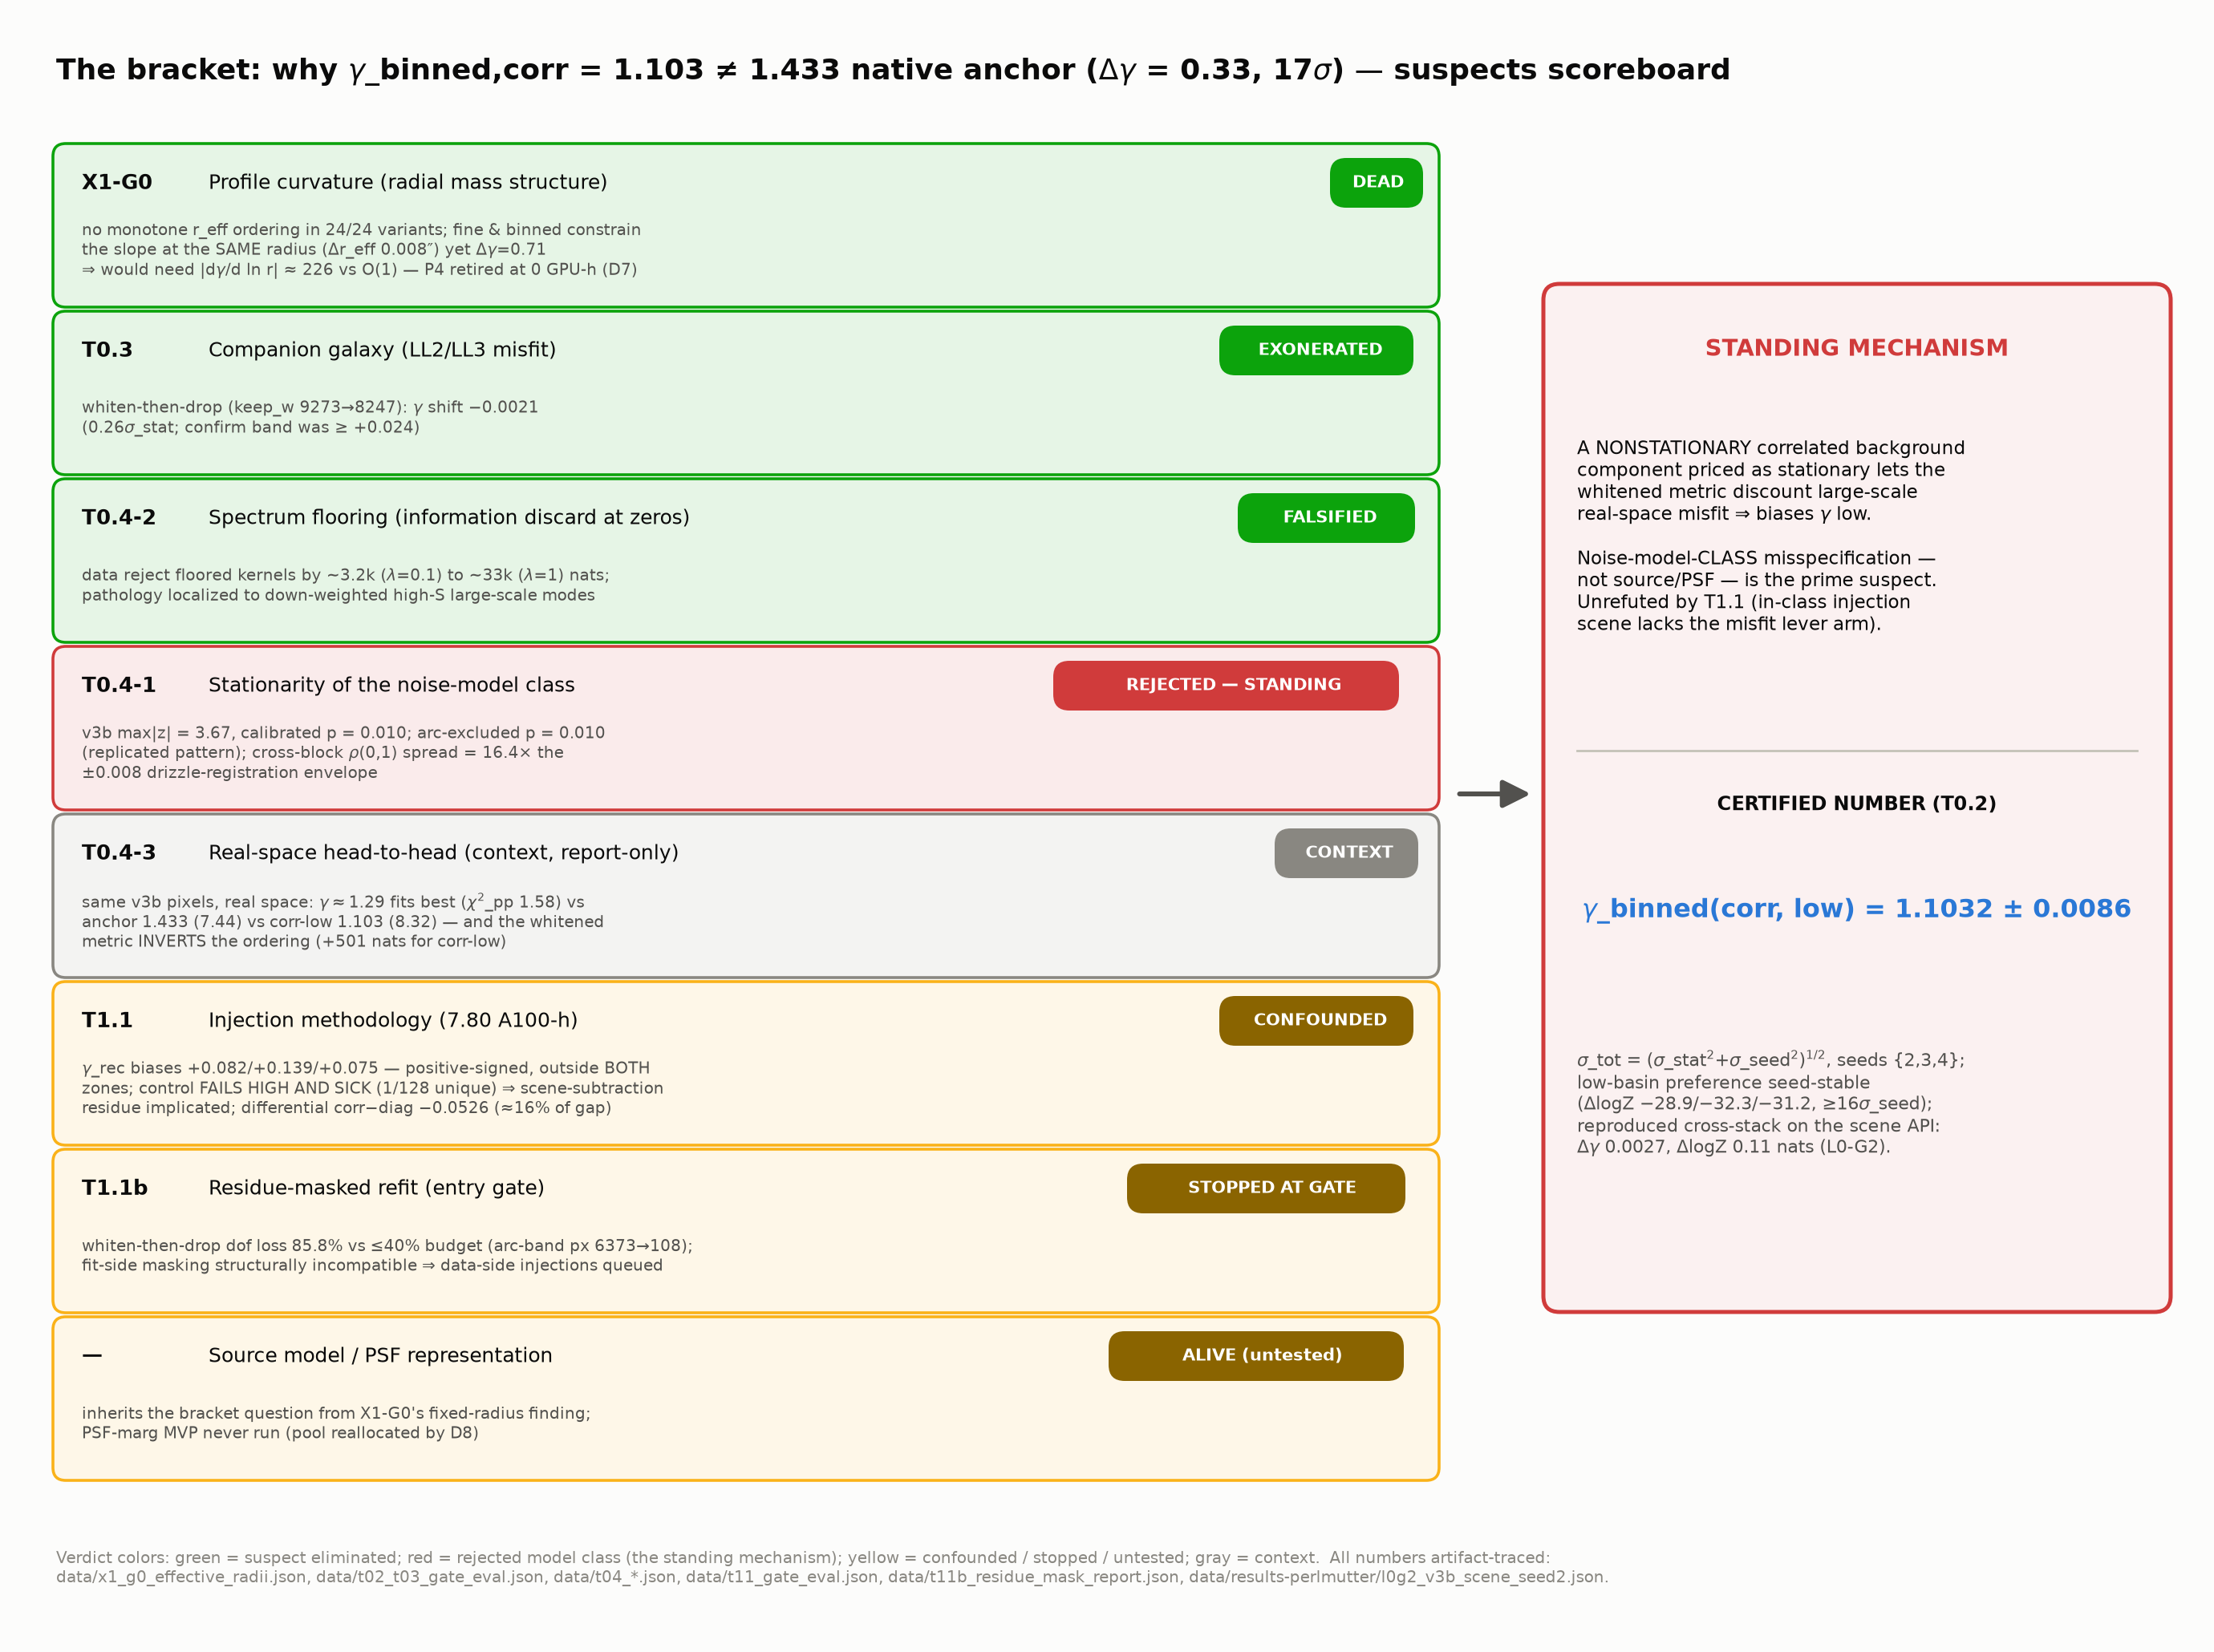
\includegraphics[width=0.98\textwidth]{../figs/rfig_bracket_scoreboard.png}
\caption{The bracket suspects scoreboard (the graphical form of
Table~\ref{tab:suspects}): one card per pre-registered discriminating
measurement, in program order. Profile curvature DEAD (X1-G0 entry-gate
kill executed as written; P4 retired at zero GPU cost, decision D7);
companion EXONERATED (T0.3); spectrum flooring FALSIFIED by
3.2k--33k~nats (T0.4-2); stationarity of the noise-model class REJECTED
at calibrated $p=0.010$ --- the standing mechanism (T0.4-1); the
real-space head-to-head as context (T0.4-3; the anchor row carries a
cross-product resolution handicap --- honest caveat);
injection--recovery CONFOUNDED by scene-subtraction residue under its
pre-registered honesty clause (T1.1, $n{=}3$, no coverage claims); the
residue-masked refit stopped at its entry gate (T1.1b, 0 A100-h);
source/PSF representation ALIVE (untested).
$\gammaEPL=1.1032\pm0.0086$ is certified (T0.2) and reproduced
cross-stack (L0-G2); the E3 kernel-scan deferral remains the standing
caveat on absolute-$\gammaEPL$ claims. Sources: the per-suspect
artifacts cited in the subsections of this section.}
\label{fig:bracket}
\end{figure}

\subsection{The number under interrogation: $\gammaEPL$ certified at
            $1.1032\pm0.0086$, with a seed-stable basin preference}
\label{sec:t02}

Before interrogating the binned-correlated slope, the campaign certified it
(T0.2: three matched-seed repeats of the production 128-particle tempered-SMC
fit on \dfile{v3b}, seeds $\{2,3,4\}$; 2.21 A100-h with
T0.3).\art{data/t02\_t03\_gate\_eval.json} The low-basin medians are
$\{1.1032,\,1.0967,\,1.1005\}$, giving $\sigma_{\rm seed}(\gammaEPL)=0.00325$
--- the pre-registered kill ($\sigma_{\rm seed}>0.024$) is not tripped ---
and
\begin{align*}
  \gammaEPL^{\rm binned}({\rm corr,\ low}) &\;=\; 1.1032 \pm 0.0086,\\
  \sigma_{\rm tot}\;=\;\sqrt{\sigma_{\rm stat}^2+\sigma_{\rm seed}^2}
  &\;=\;\sqrt{0.0080^2+0.00325^2}\;=\;0.00864\;\approx\;1.08\,\sigma_{\rm stat}.
\end{align*}
The steep basin repeats at $\{2.6393,\,2.6522,\,2.6485\}$
($\sigma_{\rm seed}=0.00664$), and the per-matched-seed basin evidence gap
$\Delta\log Z({\rm steep}-{\rm low}) = -28.88/-32.27/-31.19$~nats is
\textbf{seed-stable in sign and magnitude} --- a low-basin preference
$\ge16\,\sigma_{\rm seed}$ from zero, with
$\sigma_{\rm seed}(\Delta\log Z)=1.79$~nats
(Fig.~\ref{fig:t02}). That last number is load-bearing: the campaign's
cross-cutting finding that bootstrap errors understate evidence error makes
this measured seed scatter the honest unit for every downstream
$\Delta\log Z$ gate. Caveat, quoted with every use: $n=3$ seeds, so the
$\sigma$ estimates themselves carry $\pm46\%$ sampling error
($\chi$-distribution). Downstream thresholds were re-parameterized from the
measured $\sigma_{\rm seed}$ at this point --- a ledgered finalization, not a
goalpost move.

\begin{figure}[htbp]
\centering
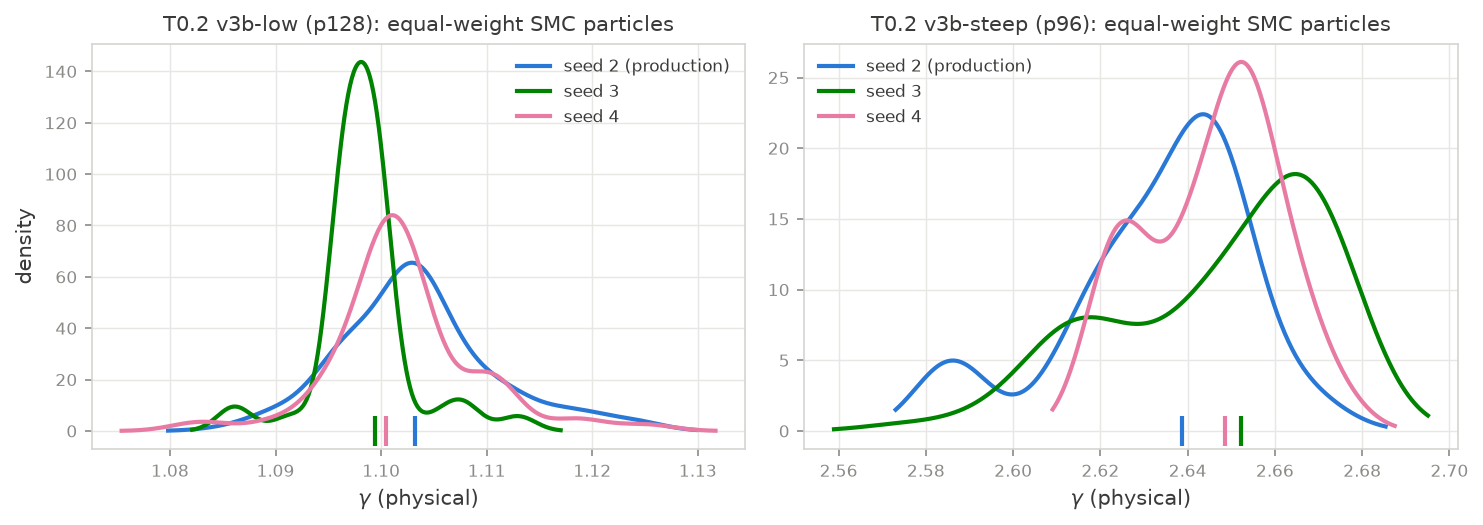
\includegraphics[width=0.9\textwidth]{../figs/t02_seed_overlay.png}
\caption{T0.2 seed-repeat certification: low- and steep-basin
$\gammaEPL$ posteriors for seeds $\{2,3,4\}$ (production tempered SMC,
\dfile{v3b} correlated likelihood). The money number is
$\gammaEPL=1.1032\pm0.0086$ ($\sigma_{\rm tot}$, seed scatter folded in);
the basin preference $\Delta\log Z({\rm steep}-{\rm low})\approx-29$ to
$-32$~nats is seed-stable. Source:
\dfile{data/t02\_t03\_gate\_eval.json}.}
\label{fig:t02}
\end{figure}

\subsection{X1-G0: profile curvature is structurally dead}
\label{sec:x1g0}

The P4 hypothesis held that the EPL single-power-law assumption drives the
bracket: whitening and binning re-weight spatial frequencies, so each product
constrains the slope at a different effective radius, and a curved
$\kappa(r)$ then yields different local slopes. Its pre-registered entry gate
(X1-G0, zero GPU cost) required the per-product effective radii to be
monotone in the same sense as the $\gammaEPL$ ordering. \textbf{The gate
failed in all 24 analysis variants} (3 statistics $\times$ primary weighting
plus 7 robustness variants), and P4 was retired unspent on the strength of
it (decision D7).\art{data/x1\_g0\_effective\_radii.json;
research/x1\_g0\_mechanism\_check.md}

\begin{table}[htbp]
\centering
\caption{X1-G0: slope-information effective radii by product
(arc-brightness $\times$ $(S/N)^2$ weighting; three statistics agree).
The required ordering ($\gammaEPL$: $1.816>1.433>1.103$) would need
$r_{\rm eff}$ monotone in the same sense; observed is
\dfile{v3} $>$ \dfile{v3b} $>$ \dfile{v2d} --- the middle-$\gammaEPL$ product
has the \emph{smallest} $r_{\rm eff}$. Source:
\dfile{data/x1\_g0\_effective\_radii.json}.}
\label{tab:x1g0}
\small
\begin{tabular}{lcccc}
\toprule
product (likelihood) & $\gammaEPL$ & $r_{\rm eff}$ mean & log-mean & median \\
\midrule
\dfile{v3} fine $0.04''$ (correlated) & $1.816\pm0.117$ & $2.596''$ & $2.578''$ & $2.613''$ \\
\dfile{v2d} native $0.13''$ (diagonal, anchor) & $1.433\pm0.035$ & $2.501''$ & $2.466''$ & $2.543''$ \\
\dfile{v3b} binned $0.08''$ (correlated) & $1.103\pm0.008$ & $2.588''$ & $2.571''$ & $2.612''$ \\
\bottomrule
\end{tabular}
\end{table}

The \textbf{fixed-radius magnitude argument} is stronger than the ordering
kill. The fine and binned products are the same sky, and their slope
information peaks at the same radius: $\Delta r_{\rm eff}\approx0.008''$
($r_{\rm mean}$ $2.5964''$ vs.\ $2.5882''$), less than a quarter of a fine
pixel --- yet their slopes differ by $\Delta\gammaEPL=0.71$. For any curved
$\kappa(r)$ to carry that gap across that lever arm would require a
local-slope gradient
$|d\gamma_{\rm loc}/d\ln r| \approx 226$ per $e$-fold; physical profile
curvature (NFW at $r_s$, dPIE break) delivers $O(1)$, and even the most
charitable product pairing needs $\approx10$
(Fig.~\ref{fig:x1g0}). The positive content of the kill: \emph{the bracket
driver differs between likelihoods at fixed radial information} --- it must
live in the noise/likelihood treatment or in source/PSF structure, not in
the radial mass profile. What the gate does \emph{not} kill: a BPL/dPIE fit
could still win on evidence for other reasons; the pre-registered
\emph{mechanism} is what is excluded.

\begin{figure}[htbp]
\centering
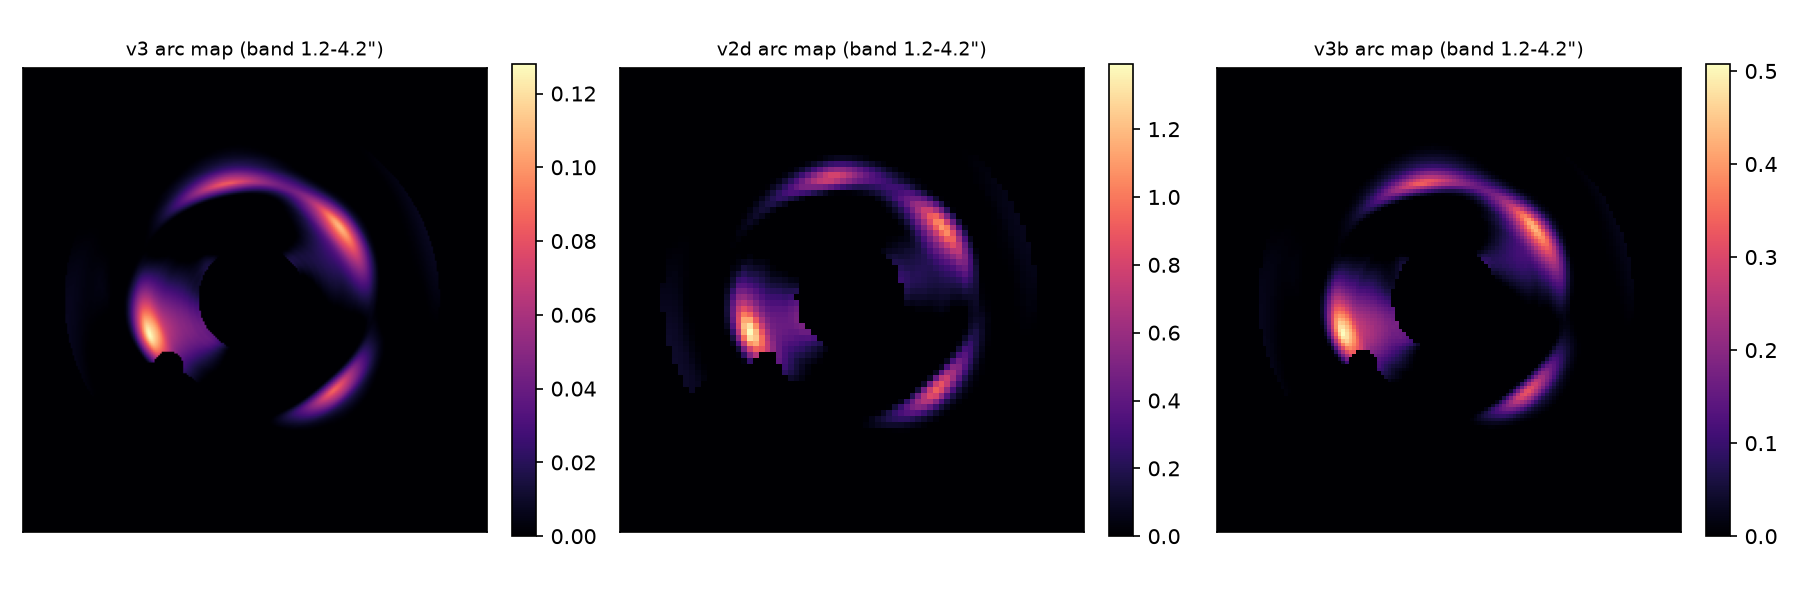
\includegraphics[width=0.92\textwidth]{../figs/x1_g0_arc_maps.png}\\[3pt]
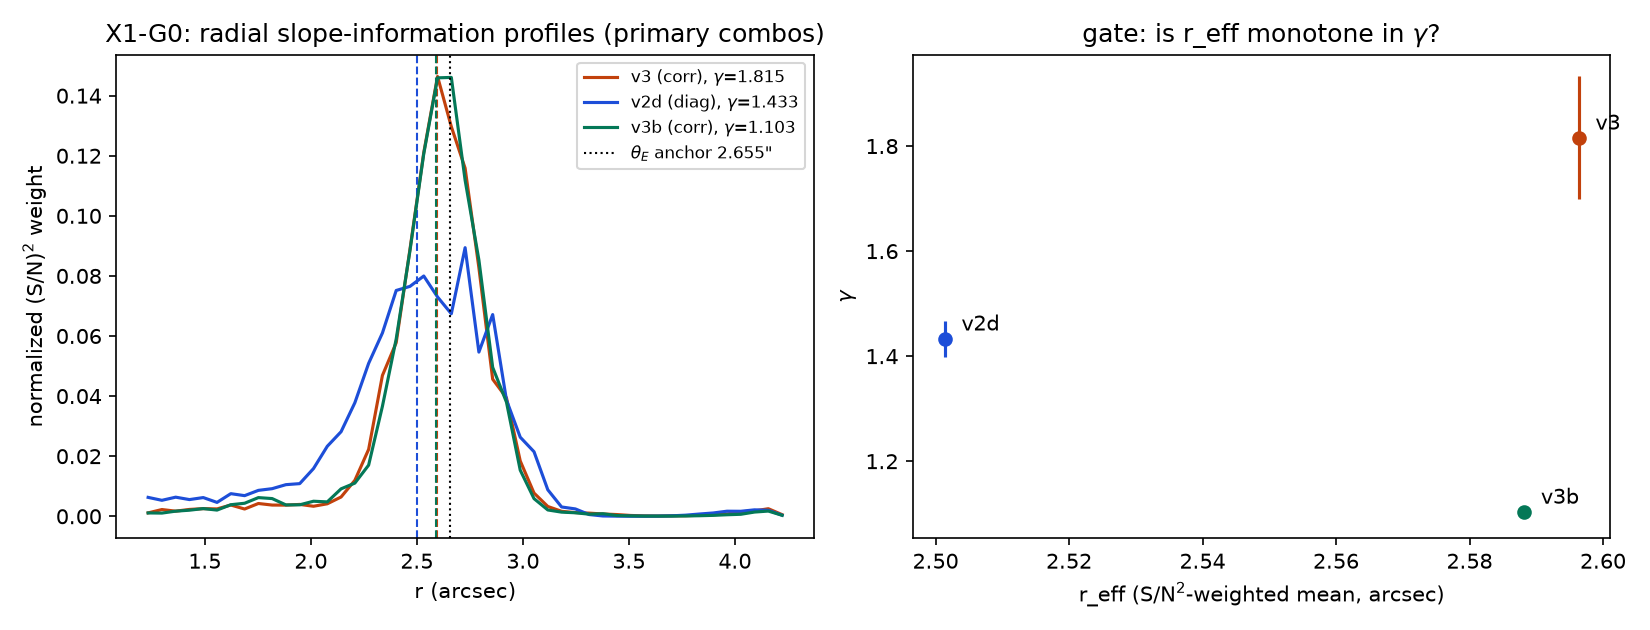
\includegraphics[width=0.92\textwidth]{../figs/x1_g0_radial_profiles.png}
\caption{X1-G0 entry-gate kill. Top: arc-brightness $\times$ $(S/N)^2$
slope-information weight maps for the three products. Bottom: radial
$(S/N)^2$ slope-information profiles (left) and the
$\gammaEPL$-vs-$r_{\rm eff}$ gate
panel (right): no monotone ordering exists (24/24 variants), and the
fine/binned pair constrains the slope at the same radius
($\Delta r_{\rm eff}\approx0.008''$) while disagreeing by
$\Delta\gammaEPL=0.71$. Source: \dfile{data/x1\_g0\_effective\_radii.json}.}
\label{fig:x1g0}
\end{figure}

\subsection{T0.3: the companion galaxy is exonerated}
\label{sec:t03}

The companion galaxy (the LL2/LL3 light components, a known local misfit) was
a candidate driver of the low slope. The pre-registered discriminator
whitens first and then drops the companion's whitened pixels (keeping the
production whitener fixed; $9273\to8247$ whitened dof), so the test isolates
the companion's likelihood contribution without rebuilding the noise model.
Result: $\gammaEPL = 1.1011$ vs.\ production $1.1032$ --- a shift of
$-0.0021$ ($0.26\,\sigma_{\rm stat}$), statistically zero against the
pre-registered detection band of $\ge+0.024$, with convergence diagnostics
indistinguishable from production.\art{data/t02\_t03\_gate\_eval.json (t03)}
\textbf{The companion is exonerated}; the noise-model class keeps its place
as prime suspect. (The companion run's $\log Z$ is not comparable to
production --- different data after the drop --- and is not used.)

\begin{figure}[htbp]
\centering
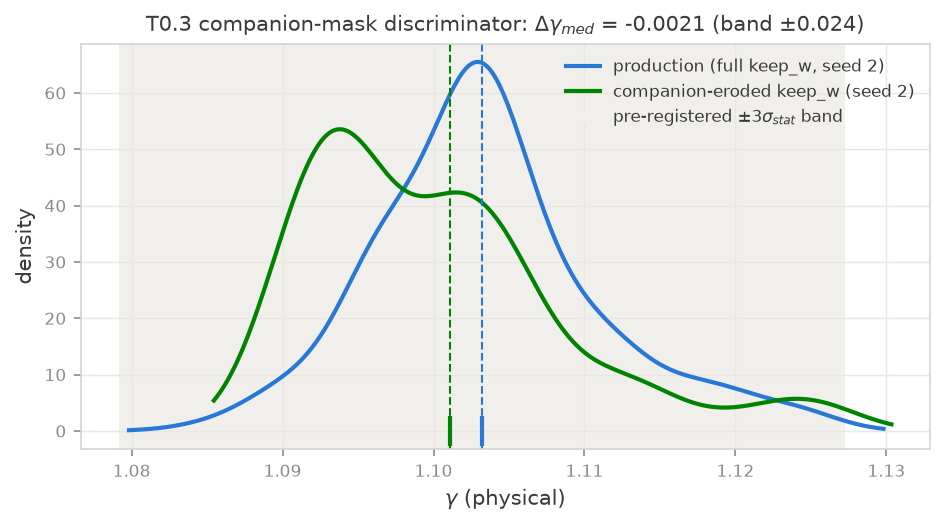
\includegraphics[width=0.62\textwidth]{../figs/t03_compmask_overlay.png}
\caption{T0.3 companion-mask discriminator: the $\gammaEPL$ posterior
under the production whitener with and without the companion's whitened
pixels ($9273\to8247$ dof). The shift is $-0.0021$
($0.26\,\sigma_{\rm stat}$) against a pre-registered detection band of
$\ge+0.024$: the companion is exonerated. Source:
\dfile{data/t02\_t03\_gate\_eval.json}.}
\label{fig:t03}
\end{figure}

\subsection{The T0.4 trilogy: the noise-model class is the standing suspect}
\label{sec:t04}

Three zero-GPU checks on the real field, run on the validated stack with
pre-registered forks, converge on one mechanism.

\subsubsection{Stationarity of the noise-model class: REJECTED}
\label{sec:t041}

The correlated likelihood behind $\gammaEPL=1.103$ prices noise with a
\emph{single stationary convolution kernel per product}. T0.4-1 tests that
class directly: per-block kernel fits on a $3\times3$ grid over the field,
with null bands calibrated by 200 exact FFT resamples of stationary fields
under the global fitted kernel (mask geometry and finite-block scatter
included), and a multiplicity-honest calibrated $p$ from the same
max$|z|$ statistic on every null draw.\art{data/t04\_stationarity.json;
data/t04\_stationarity\_noarc.json} The verdict
(Fig.~\ref{fig:stationarity}):

\begin{itemize}
\item The money product \dfile{v3b} rejects the stationary class at
$\max|z|=3.67$, \textbf{calibrated $p=0.010$}; the arc-excluded \dfile{v3}
robustness arm also rejects at $p=0.010$ ($\max|z|=3.66$) --- excluding the
arc band \emph{strengthens} the fine-product rejection (arc residuals were
diluting the signal, not driving it).
\item The rejection is a coherent, cross-product-replicated spatial pattern
--- top row of blocks over-correlated ($\rho(0,1)$ up to $0.71$ vs.\ global
$0.60$), middle-left block under-correlated ($z$ down to $-3.7$) --- the same
sign pattern in \dfile{v3} and \dfile{v3b}, with and without the arc band.
That is what a real shift-variant noise field predicts and a fit fluke does
not.
\item Drizzle sub-pixel registration cannot explain it: the enumerated
registration envelope predicts a block-to-block $\rho(0,1)$ spread of
$\pm0.008$; the observed spread is $\sim$$0.28$ peak-to-peak on \dfile{v3b}
--- \textbf{$16.4\times$ the envelope}. The nonstationarity must come from
something else that varies across the skycell (coverage/weight-map
structure and/or residual astrophysical background).
\end{itemize}

\textbf{The noise-model class that produced $\gammaEPL=1.103$ is provably
violated by the field it whitens.} Honest caveats: the four test arms share
pixels and are not independent --- the case is the replicated pattern, not
any single $p$-value.

\begin{figure}[htbp]
\centering
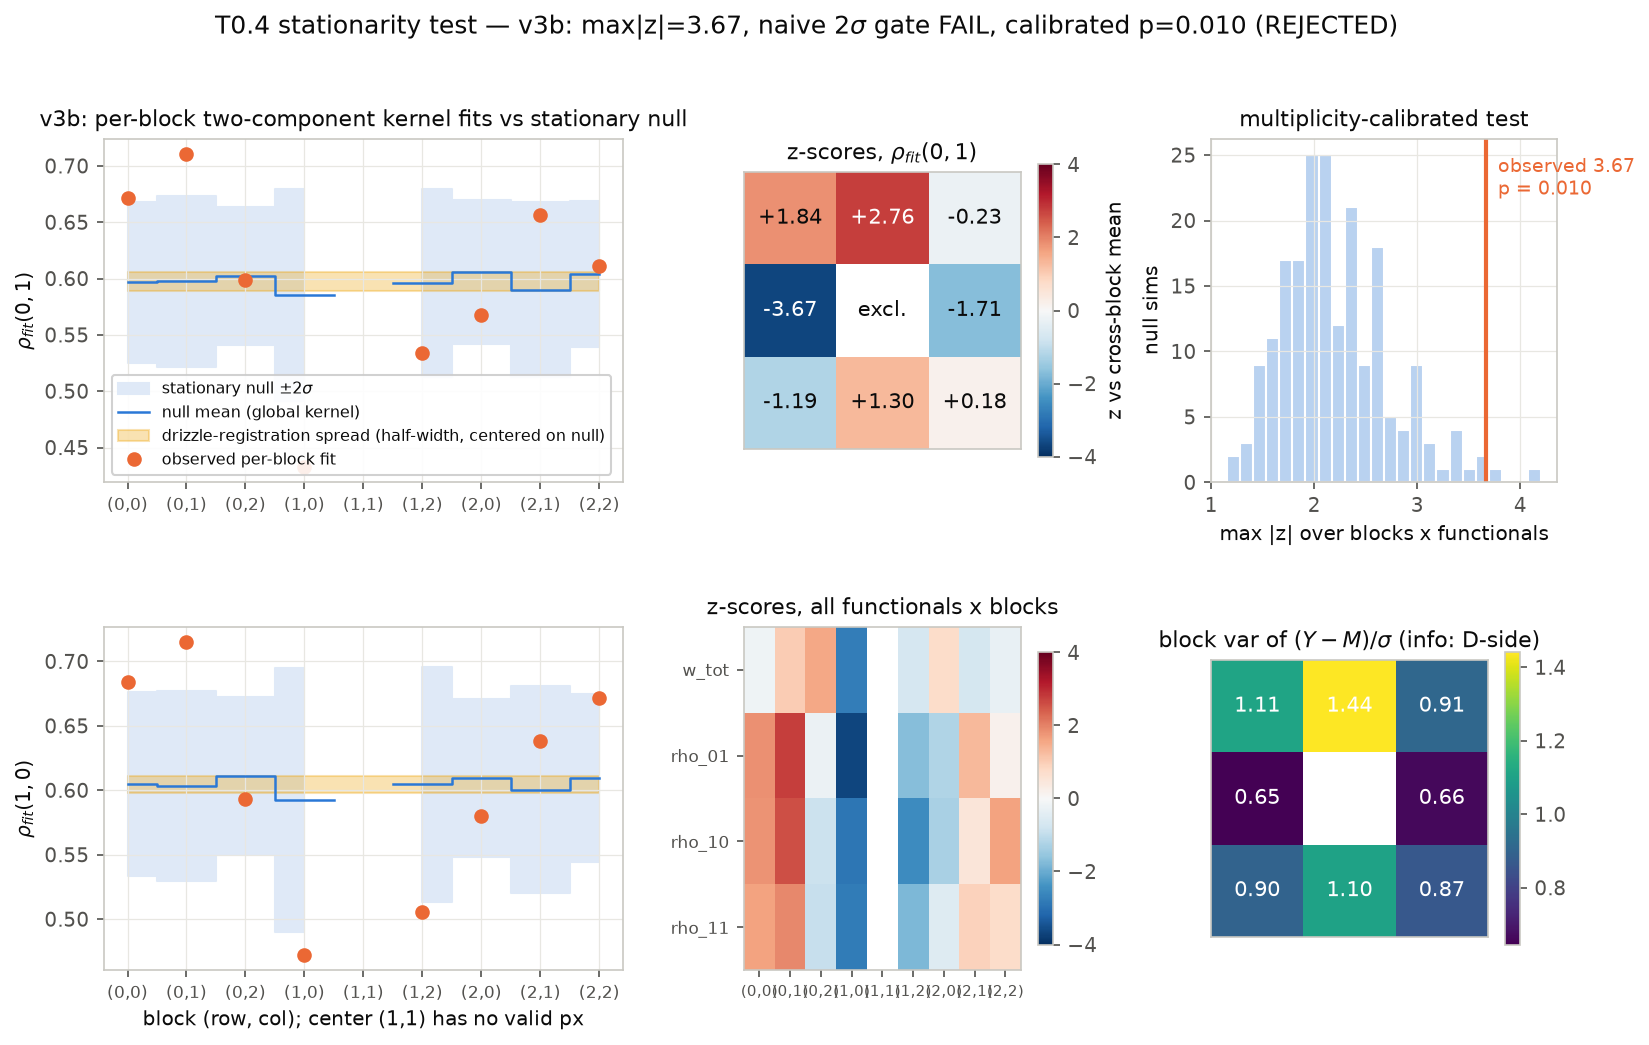
\includegraphics[width=0.78\textwidth]{../figs/t04_stationarity_v3b.png}\\[3pt]
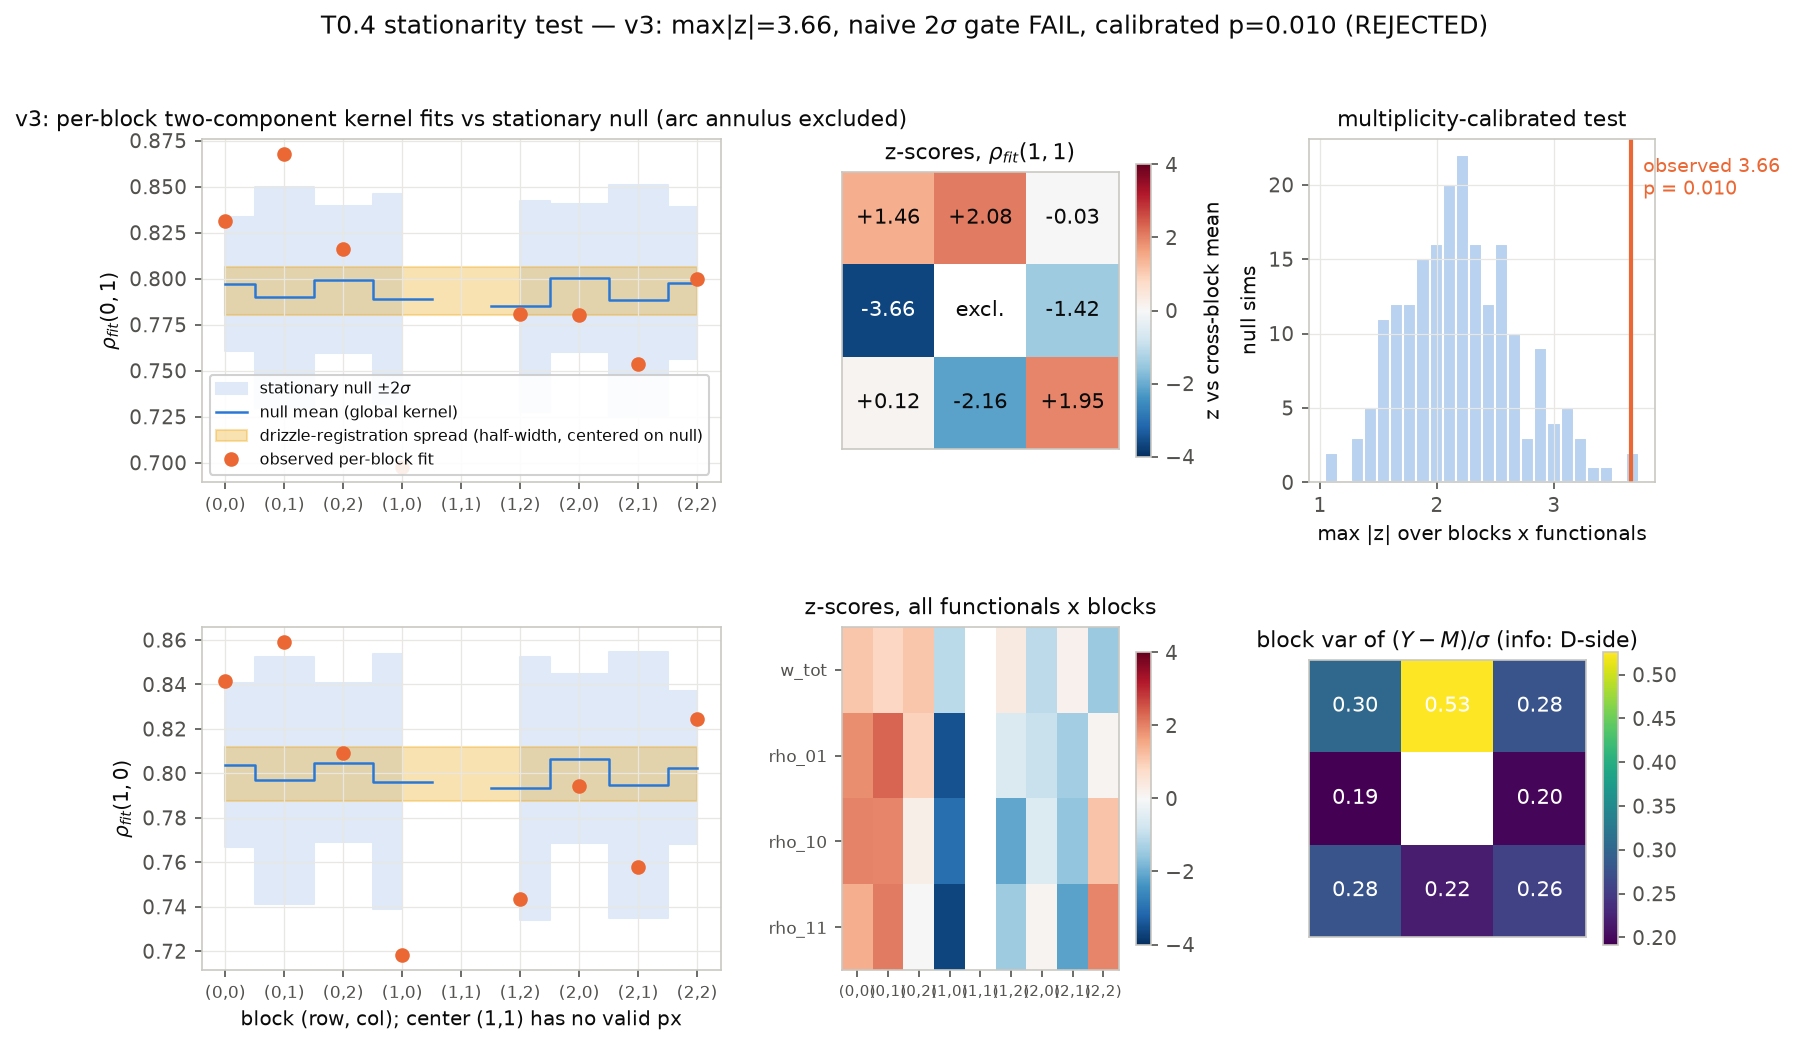
\includegraphics[width=0.78\textwidth]{../figs/t04_stationarity_v3_noarc.png}
\caption{T0.4-1 stationarity rejection. Top: the money product \dfile{v3b}
--- per-block kernel functionals vs.\ null-calibrated bands
($\max|z|=3.67$, calibrated $p=0.010$). Bottom: the arc-excluded fine
product \dfile{v3} ($\max|z|=3.66$, $p=0.010$) --- excluding the arc band
\emph{strengthens} the fine-product rejection (with the arc included,
\dfile{v3} gives $p=0.17$). The spatial pattern (top row over-correlated,
middle-left under-correlated) replicates across products and pixel-set
arms; its amplitude is $16.4\times$ the drizzle-registration envelope.
Sources: \dfile{data/t04\_stationarity.json};
\dfile{data/t04\_stationarity\_noarc.json}.}
\label{fig:stationarity}
\end{figure}

\subsubsection{Spectrum flooring: FALSIFIED as mechanism and as cure}
\label{sec:t042}

A proposed benign reading of the low slope was information discard at
spectral zeros: the near-singular fine whitener amplifies low-power modes,
and flooring the whitener spectrum (raising $s_{\rm floor}=\lambda$) should
then cure the known ``fine-low gaming'' pathology, in which optimization
drives $\gammaEPL\to1.02$ while whitened log-probability improves and
real-space $\chi^2$ collapses. T0.4-2 rebuilt the whitener across
$\lambda\in\{0.05\ (\equiv{\rm production,\ unfloored}),0.1,0.3,1.0\}$ ---
the production build is reproduced to $\max|\Delta h|=1.0\times10^{-9}$ in
the taps, and the production floor is $s_{\rm floor}=0.05$, at which the
floor does not engage (the plan's ``0.1'' label is corrected in the
artifact) --- and scored three frozen points (the v3b-low start~A, the
railed fine-low MAP~B, the fine-steep MAP~C) under exact cross-$\lambda$
normalization ($\log|C(\lambda)|$ via Szeg\H{o}, dense-Cholesky anchored to
$\le7\times10^{-4}$~nat/px).\art{data/t04\_lambda\_arm.json}

Two results (Fig.~\ref{fig:lambdaarm}):
\begin{itemize}
\item \textbf{Flooring never re-aligns the orderings.} The
whitened-vs-real-space inversion (B beats A by $\sim$4200 whitened nats at
production while real space prefers A by $\Delta\chi^2_{\rm pp}=37$)
persists essentially unchanged from the unfloored whitener through
$\lambda=1.0$ (85\% of modes floored): still $+3832$~nats. If the pathology
lived at the spectral zeros, flooring them would have fixed it.
\item \textbf{The data reject the floored kernels outright}: the normalized
likelihood drops by $\sim$3.2k~nats per point at $\lambda=0.1$
($-3187/-3328/-3304$ for A/B/C) and by $\sim$33k~nats at $\lambda=1.0$
($-33{,}060/-33{,}450/-33{,}370$). ``Cure by flooring'' costs thousands of
nats of evidence per step --- more than any plausible model could repay.
\end{itemize}

The pathology is localized instead in what flooring never touches: the
\emph{down-weighting of high-power large-scale modes}
($S_{\max}/{\rm mean}\approx99$ --- the fitted correlated-background
component, $w_b\approx0.27$), which prices large-scale real-space residual
structure at $\sim$1/10 amplitude weight. Those are exactly the modes
T0.4-1 shows are nonstationary: the two checks indict the same component.

\begin{figure}[htbp]
\centering
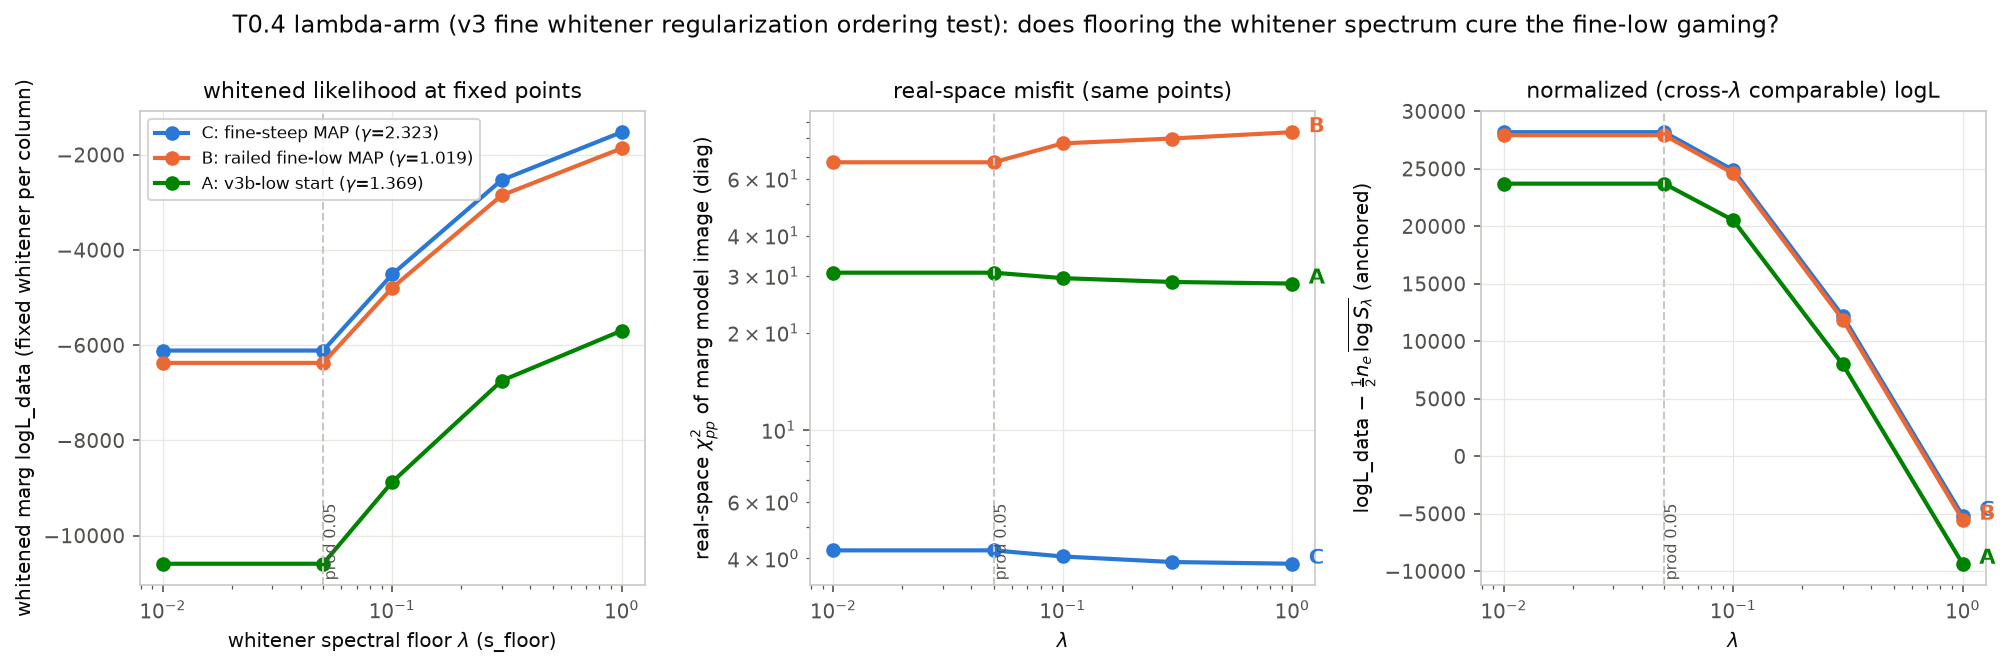
\includegraphics[width=0.9\textwidth]{../figs/t04_lambda_arm.png}
\caption{T0.4-2 $\lambda$-arm: whitened and normalized likelihoods of the
three frozen points vs.\ spectrum floor $\lambda$. The gaming inversion is
flat in $\lambda$ (flooring does not cure it) while the normalized
likelihood rejects the floored kernels by $3.2$k--$33$k~nats per point.
Source: \dfile{data/t04\_lambda\_arm.json}.}
\label{fig:lambdaarm}
\end{figure}

\subsubsection{Real space vs.\ the whitened metric: the orderings invert}
\label{sec:t043}

T0.4-3 (report-only by design, a free ordering check rather than a
calibrated test) asks which solution the binned pixels themselves prefer in
plain real space. Forward renders of three on-disk posterior medians on the
\emph{same} \dfile{v3b} pixels, each given its ridge-solved (real-space
optimal) source amplitudes:\art{data/t04\_realspace\_headtohead.json}

\begin{table}[htbp]
\centering
\caption{T0.4-3 real-space head-to-head on the same \dfile{v3b} binned
pixels (diag-solved source amplitudes; 16{,}653 keep px full field, 7{,}825
px arc band $r\in[1.2,4.2]''$). The production whitened metric inverts the
real-space ordering. Source: \dfile{data/t04\_realspace\_headtohead.json}.}
\label{tab:headtohead}
\small
\begin{tabular}{lcccc}
\toprule
model ($\gammaEPL$) & $\chi^2_{\rm pp}$ full & $\chi^2_{\rm pp}$ arc band &
whitened $\log L_{\rm data}$ & whitened log-posterior \\
\midrule
anchor $1.433$ (from \dfile{v2d}) & $7.44$ & $3.62$ & $-5442.1$ & $-5615.7$ \\
corr-low $1.103$ (money) & $8.32$ & $2.76$ & $\mathbf{-4599.2}$ & $\mathbf{-4683.6}$ \\
diag-low $1.293$ (home reference) & $\mathbf{1.58}$ & $\mathbf{1.93}$ & $-4662.3$ & $-5184.3$ \\
\bottomrule
\end{tabular}
\end{table}

In real space the binned data's preference is the home-product diagonal-low
solution at $\gammaEPL\approx1.29$ ($\chi^2_{\rm pp}$ $1.58$ full / $1.93$
arc band); the $1.103$ corr-low model is real-space poor ($8.32$ / $2.76$),
its residual dominated by smooth lens-center misfit --- the same currency as
the fine-low gaming. \textbf{The production whitened metric inverts this
ordering}, preferring corr-low over diag-low by $+63$~nats in
$\log L_{\rm data}$ and \textbf{$+501$~nats in log-posterior}. The $1.103$
solution is a whitened-metric optimum, not a real-space one, \emph{on its
own product}. Honest caveat on the anchor row: its full-field number
carries a cross-product resolution handicap (parameters fit at $0.13''$
rendered at $0.08''$; the same point renders $\chi^2_{\rm pp}=1.25$ on its
home product), so the defensible summary is that \emph{neither} extreme-%
$\gammaEPL$ model is the binned data's real-space preference --- the
$\gammaEPL\approx1.29$ diagonal solution is (Fig.~\ref{fig:headtohead}).

\begin{figure}[htbp]
\centering
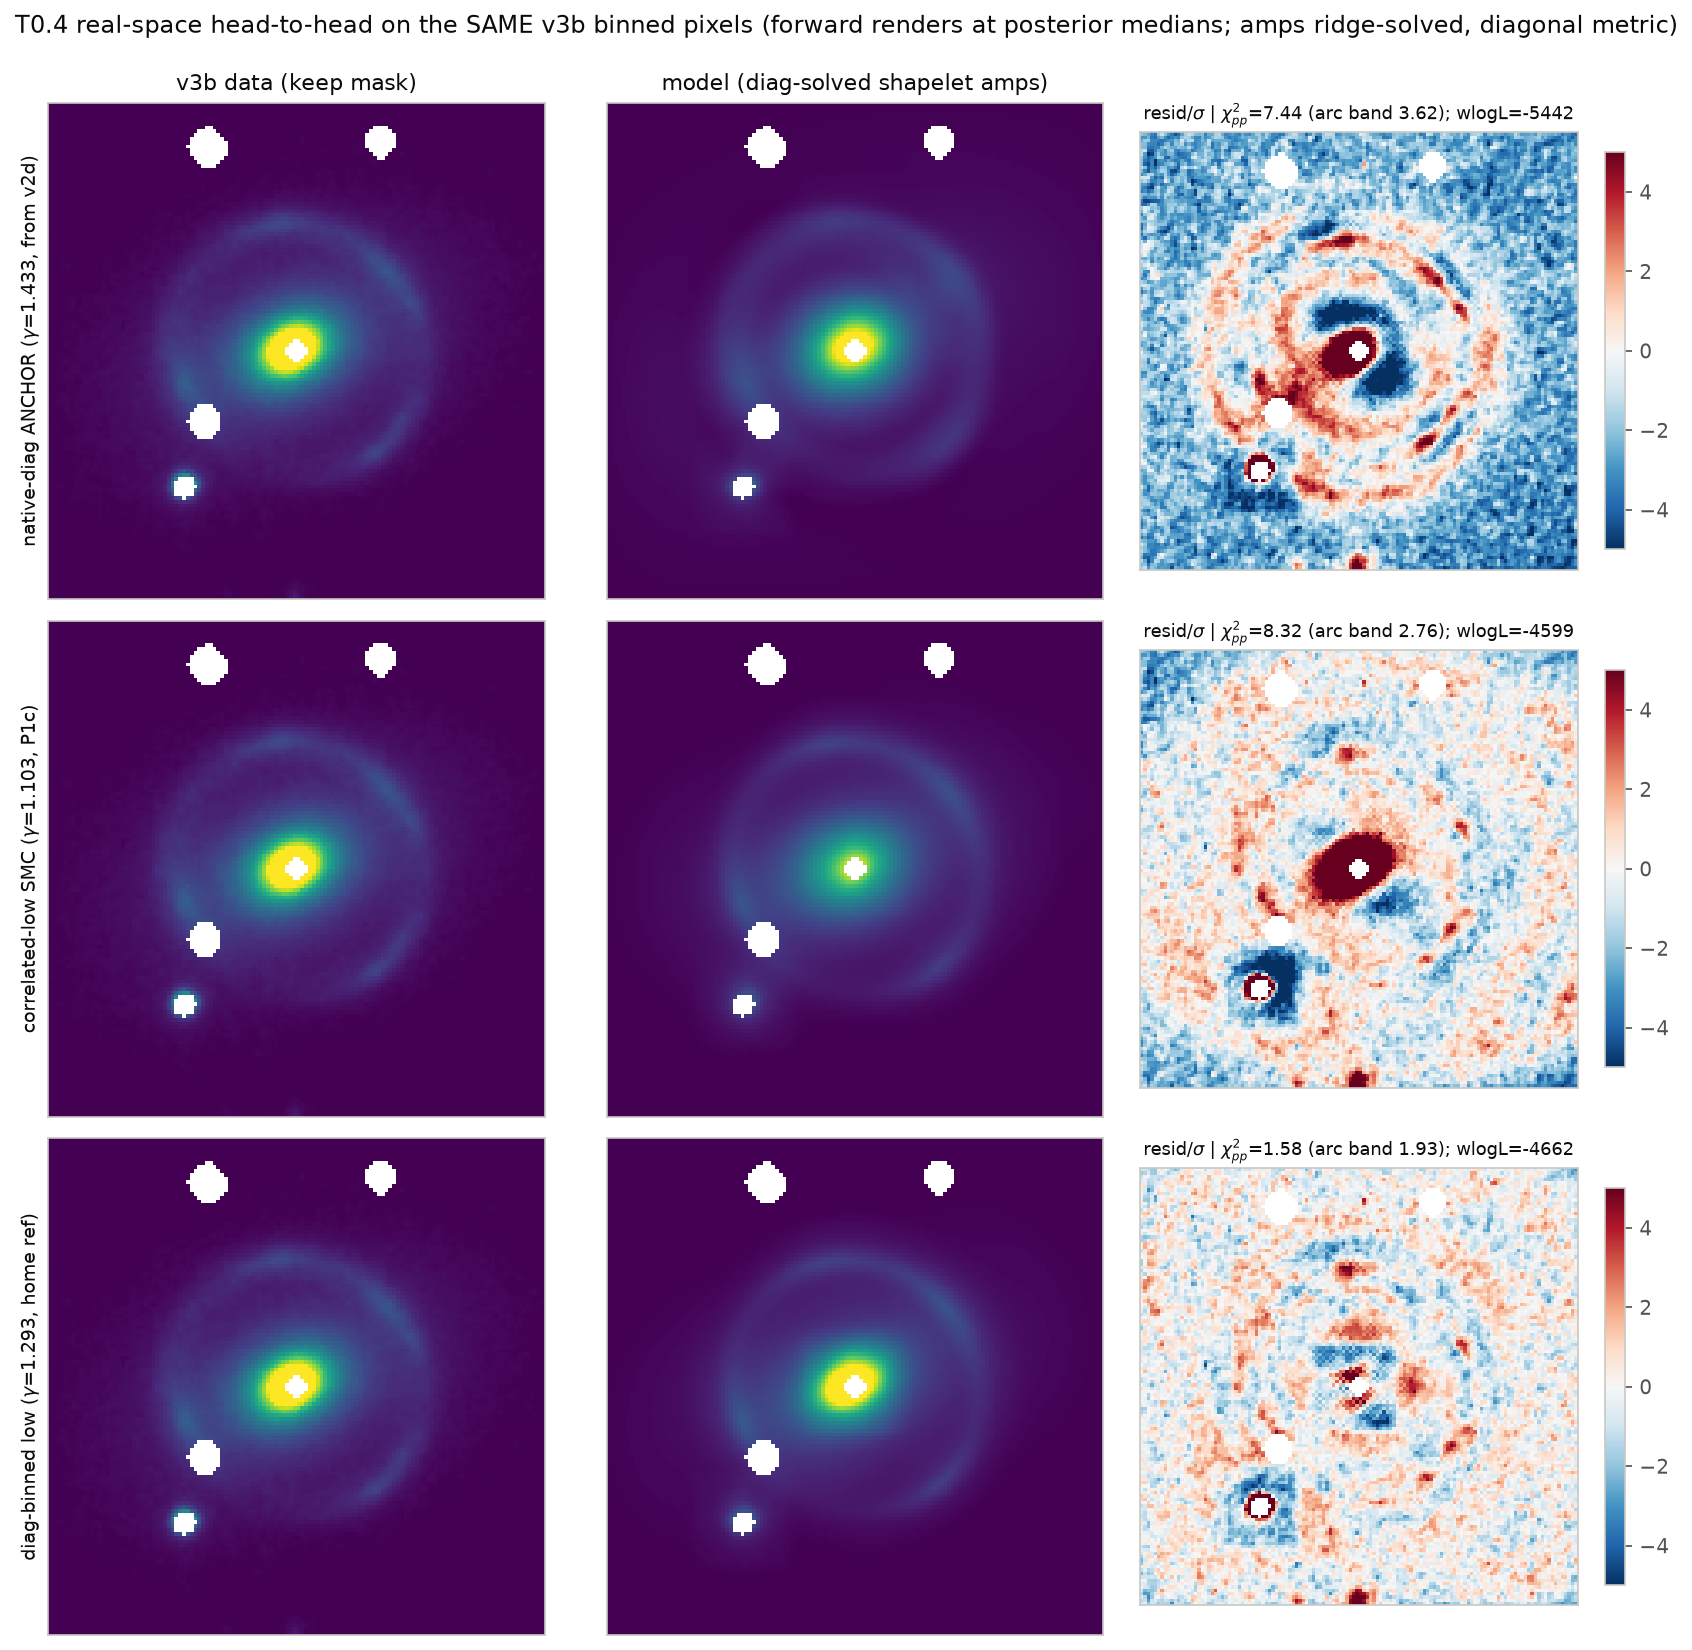
\includegraphics[width=0.92\textwidth]{../figs/t04_headtohead_residuals.png}
\caption{T0.4-3 residual maps on the same \dfile{v3b} pixels for the three
posterior medians. The corr-low ($\gammaEPL=1.103$) render leaves strong
coherent lens-center residuals that the whitened metric prices as
``probably correlated noise''; real space prefers the
$\gammaEPL\approx1.29$ diagonal solution. Source:
\dfile{data/t04\_realspace\_headtohead.json}.}
\label{fig:headtohead}
\end{figure}

\medskip\noindent\textbf{Mechanism synthesis (working hypothesis, not a
conviction).} One mechanism spans all of T0.4 and the X1-G0 constraint: the
fitted stationary kernels contain a large correlated-background component
($w_b\approx0.25$--$0.27$) estimated from sky that is provably \emph{not}
stationary across the field; the whitener therefore prices large-scale
real-space misfit at $\sim$1/10 weight everywhere, including regions where
that pricing is wrong; solutions that spend exactly this currency
(fine-low gaming, the $1.103$ optimum) become whitened-optimal while real
space disagrees --- a coherent route to a low-biased $\gammaEPL$ at fixed
radial information. Noise-model-\emph{class} misspecification is thereby the
prime suspect for the $1.103$ over-correction; a locally-stationary
(per-region kernel) class is the indicated next likelihood iteration, and
the ported \texttt{CorrelatedImageData} deliberately keeps its whitener seam
pluggable for it. Standing caveat: the kernel-hyperparameter scan (E3) was
deferred by plan and never funded, and the alternative class was never
fitted --- the mechanism rests on a class-level rejection plus consistent
circumstantial evidence, and the confirmatory injection test came back
confounded, as the next subsection reports.

\subsection{T1.1: injection--recovery is confounded --- an honest negative}
\label{sec:t11}

T1.1 was the mechanism's confirmatory experiment (7.80 A100-h; jobs
55952480/55952481/55958518 + diagonal control 55952483): inject arcs of
known slope $\gammaEPL_{\rm truth}=1.4330$ into the \emph{real} \dfile{v3b}
drizzle residual field at three sub-pixel shifts, refit with the production
correlated pipeline, and read the recovered slope against pre-registered
zones --- CONFIRM-low if ${\rm median}(\gamma_{\rm rec}-1.433)<-0.078$;
EXONERATE if $|{\rm median}|<0.026$; a diagonal-likelihood control on the
same data predicted in
$[1.29,1.43]$.\art{data/t11\_gate\_eval.json;
research/t11\_injection\_recovery.md}

\textbf{The result lands outside both zones, on the positive side}
(Fig.~\ref{fig:t11}): recovered medians $1.5151/1.5719/1.5076$, biases
$+0.0822/+0.1389/+0.0747$ (own-$\sigma$ $z$ $+2.25/+3.23/+1.82$); median
bias $+0.0822$ ($+0.0784$ dropping the duplicate-flagged inj2 --- same
conclusion). The mechanism's directional prediction failed at face value.
\textbf{And the control failed high and sick}: $\gamma_{\rm rec}=1.5677
\notin[1.29,1.43]$, with total resample collapse (1 unique particle of 128,
$\sigma_\gamma=4\times10^{-16}$) and the injected source's amplitude railed
at $\approx58\times$ truth. Per the pre-registered honesty clause, a control
failing its own window implicates the \emph{injection construction}, not
the whitener: both likelihood classes on the same injected field recover
$\gammaEPL$ high by $+0.07$--$0.14$, the only shared element is the data,
and the real residual field carries the real lens's imperfect
bright-object scene subtraction. The nuisance readout shows exactly the
absorption signature --- recovered sources $\times1.8$--$3$ larger and
$\times2.4$ brighter than injected truth in all three correlated runs.
$n=3$; no coverage claims.

Two salvage data survive, quoted at their honest strength:
\begin{itemize}
\item \textbf{The whitener-isolating differential}: on identical data
(inj1), $\gamma({\rm corr})-\gamma({\rm diag}) = -0.0526$ --- sign
consistent with the mechanism, magnitude $\approx16\%$ of the real-data
$0.330$ gap, and \emph{no defensible error bar} (the diagonal leg is a
degenerate point mass).
\item \textbf{What T1.1 could not test by construction}: the injected scene
is exactly in-class (truth source = fitted shapelet ridge solve), so the
mechanism's lever arm --- discounted large-scale structural \emph{misfit}
--- is largely absent by design. Even a clean exonerate here would not have
refuted T0.4-1's direct stationarity rejection, which stands unrefuted.
\end{itemize}

\textbf{Verdict: NO-CONFIRM / NO-EXONERATE.} The mechanism diagnosis
continues to rest on T0.4's direct evidence; T1.1 neither strengthens nor
weakens it decisively.

\begin{figure}[htbp]
\centering
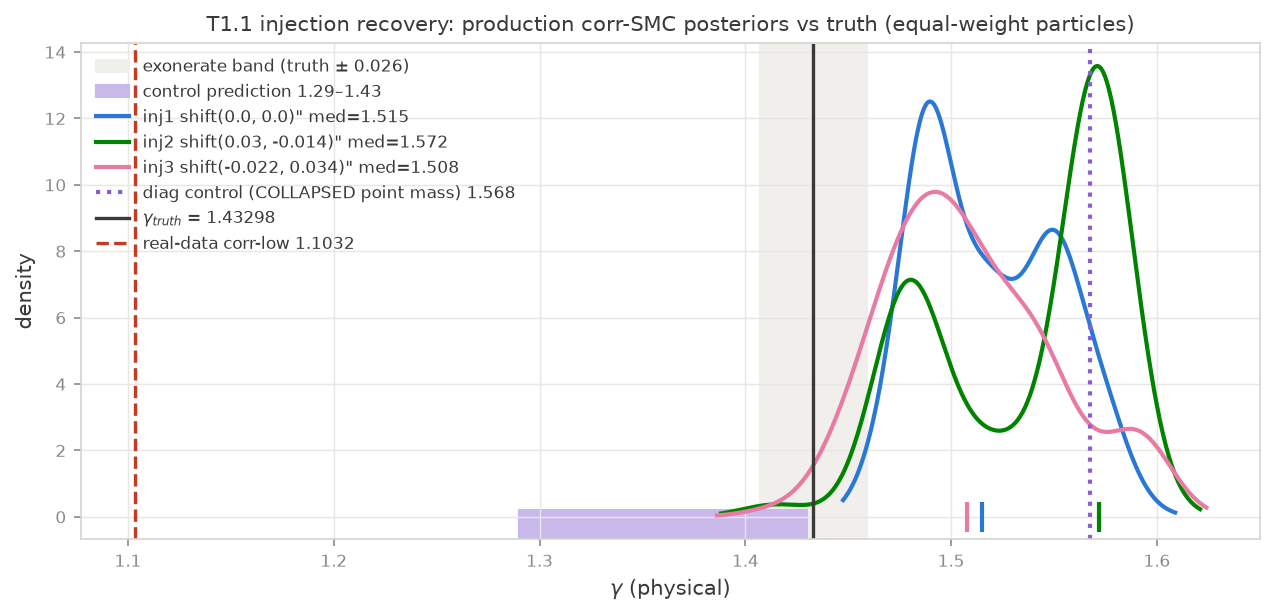
\includegraphics[width=0.9\textwidth]{../figs/t11_recovery_overlay.png}
\caption{T1.1 injection--recovery: recovered $\gammaEPL$ posteriors for the
three correlated injections and the diagonal control vs.\ the injected
truth $1.4330$ and the pre-registered zones. All arms land high (scene
residue absorption); the control is both out-of-window and degenerate.
Source: \dfile{data/t11\_gate\_eval.json}.}
\label{fig:t11}
\end{figure}

\subsection{T1.1b: the fit-side rescue fails structurally --- injections
            must be rebuilt data-side}
\label{sec:t11b}

The obvious rescue --- mask the scene-subtraction residue on the fit side
(whiten with the production kernel, then drop residue-dominated whitened
pixels) --- was given a pre-declared entry gate before any GPU spend: the
kept-dof loss had to stay $\le40\%$. \textbf{It failed structurally, and
T1.1b stopped at zero cost}: whiten-then-drop loses $85.8\%$ of the
whitened dof ($9273\to1320$; the region drop alone loses $47.6\%$), and the
arc band --- where the slope information lives --- retains 108 of 6373
whitened pixels, all outer sky.\art{data/t11b\_residue\_mask\_report.json}
The $21\times21$ whitening kernel support smears the excluded regions across
the field: fit-side residue masking is structurally incompatible with this
injection design, not merely expensive.

\textbf{The redesign conclusion is data-side}: residue-free injection
substrates must be built before whitener-bias numbers are quotable ---
kernel-sampled noise-only fields, sky-set bootstrap, or a deeper
multi-start scene subtraction. This was queued as the follow-on experiment
and remains unfunded at program close; it is the sharpest single item on
the handoff list, because it is what stands between ``indicted'' and
``convicted'' for the noise-model mechanism.

\subsection{L0-G2: $\gammaEPL=1.103$ reproduces across stacks and machines}
\label{sec:l0g2}

The final mechanism-program result is a positive control on everything
above (0.53 A100-h; job 55985451, 31 min). The ported correlated likelihood
(\S\ref{sec:corrport}) refit the \dfile{v3b} low and steep basins on the
scene-API substrate --- an independent implementation stack, on a different
machine, mirroring the production recipe at seed 2. Against the
pre-registered gate ($|\gammaEPL-1.1032|\le0.017$ and
$\Delta\log Z({\rm steep}-{\rm low})<0$), the refit
\textbf{passes}:\art{data/results-perlmutter/l0g2\_v3b\_scene\_seed2.json}

\begin{itemize}
\item $\gammaEPL_{\rm low} = 1.1005\ [1.0992, 1.1065]$, i.e.\
$\Delta=0.0027$ from the certified $1.1032$ --- well inside both the gate
and $\sigma_{\rm seed}$;
\item $\log Z_{\rm low} = -4770.97$ vs.\ the old-stack production
$-4771.08$: \textbf{0.11~nats of agreement across stacks \emph{and}
machines};
\item $\Delta\log Z({\rm steep}-{\rm low}) = -29.36$, in sign and magnitude
inside the old-stack seed family ($-28.9/-32.3/-31.2$).
\end{itemize}

The \texttt{CorrelatedImageData} port is thereby licensed at posterior
level, and $\gammaEPL=1.103$ now stands on two independent stacks --- the
over-correction of \S\ref{sec:t04} is a property of the \emph{likelihood
class}, not of either implementation. Scope notes (UNCERTIFIED---external;
proposed to the upstream team as CGL2-C5): the same frozen whitener bundle
feeds both stacks, so this is a stack-implementation cross-check, not an
independent noise model; single seed on the new stack, with the old-stack
$\sigma_{\rm seed}$ ($n=3$, $\pm46\%$) as context.

\begin{figure}[htbp]
\centering
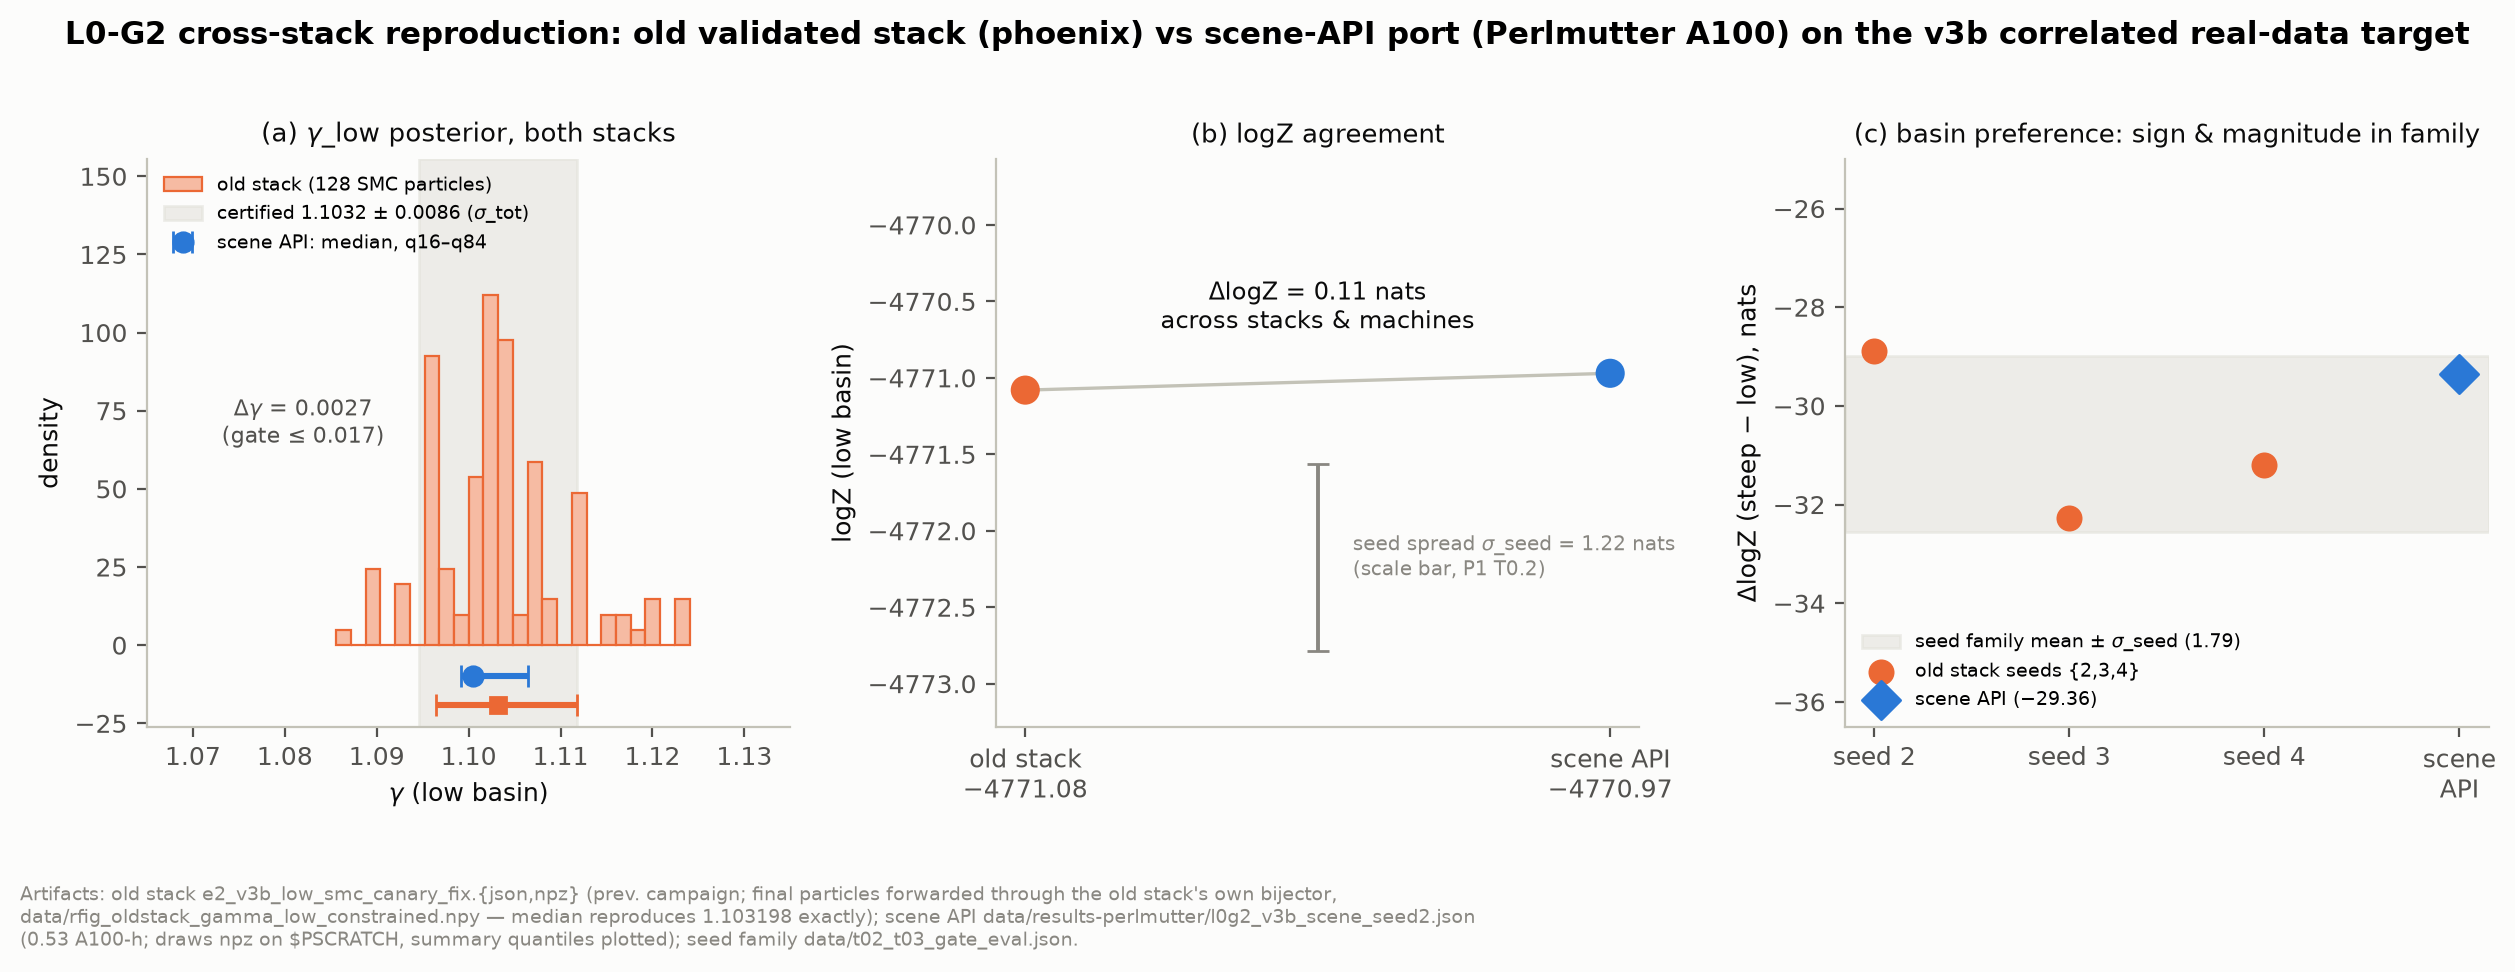
\includegraphics[width=0.98\textwidth]{../figs/rfig_crossstack_l0g2.png}
\caption{L0-G2 cross-stack reproduction of the correlated \dfile{v3b}
refit. (a) $\gammaEPL_{\rm low}$: the previous campaign's production SMC
ensemble (128 final particles, phoenix, old validated stack; particles
forwarded through that stack's own bijector --- the median reproduces the
ledgered $1.103198$ exactly) against the scene-API port's summary
quantiles (Perlmutter A100, seed 2): $\Delta\gammaEPL({\rm
median})=0.0027$, inside both the pre-registered $0.017$ gate and the
certified $1.1032\pm0.0086$ band. (b) $\log Z$ agreement to $0.11$~nats
across stacks \emph{and} machines ($-4771.08$ vs.\ $-4770.97$), with the
old-stack seed spread of $\log Z_{\rm low}$
($\sigma_{\rm seed}=1.22$~nats) as the honest scale bar (per-run
bootstrap $\sigma$ is not recorded in these summary artifacts).
(c) $\Delta\log Z({\rm steep}-{\rm low})=-29.36$ on the scene API, inside
the old-stack seed family ($-28.88/-32.27/-31.19$). The scene side is
plotted from summary quantiles (the posterior-draws NPZ resides on
Perlmutter scratch). Sources:
\dfile{data/results-perlmutter/l0g2\_v3b\_scene\_seed2.json};
\dfile{data/rfig\_oldstack\_gamma\_low\_constrained.npy};
\dfile{data/t02\_t03\_gate\_eval.json}.}
\label{fig:l0g2}
\end{figure}

%%%%%%%%%%%%%%%%%%%%%%%%%%%%%%%%%%%%%%%%%%%%%%%%%%%%%%%%%%%%%%%%%%%%%%%%%%%%%%%
\section{Results III --- Fermat-Potential Sensitivity: a Triple-Disclaimed
         Teaser}
\label{sec:fermat}
%%%%%%%%%%%%%%%%%%%%%%%%%%%%%%%%%%%%%%%%%%%%%%%%%%%%%%%%%%%%%%%%%%%%%%%%%%%%%%%

\noindent\emph{Read the disclaimers first; they are the load-bearing part of
this section.} (1)~\foundry\ is \textbf{not a time-delay lens} --- no source
variability, placeholder redshifts; nothing here is a $\Delta t$ prediction
for a real system. (2)~The image positions are \textbf{synthetic}: four
fixed points on a $\thetaE=2.655''$ circle about the anchor mass center, the
same points for every posterior. (3)~The correlated binned-low posterior is
the product \textbf{known to over-correct}
($\gammaEPL=1.103$, $17\sigma$ below the $1.433$ anchor;
\S\ref{sec:mech}) --- so this teaser demonstrates \emph{sensitivity} of
Fermat observables to the coadd-covariance modeling choice; it does
\emph{not} calibrate which answer is right. Additionally, the primary
comparison pair differs by data product (native vs.\ binned), not only by
noise model; the same-product secondary arm isolates the noise model.

\medskip
With that stated, the number (0 GPU-h; per-sample EPL+shear Fermat
potentials through a numpy port of the EPL deflection --- Tessore--Metcalf
angular series, validated against the vendored jax implementation to
$\max|\Delta|=1.3\times10^{-15}$; fractional shifts are
distance/redshift-free):\art{data/fermat\_dt\_teaser.json;
research/fermat\_dt\_teaser.md} swapping the noise model moves the median
Fermat-potential differences $\Delta\phi$ between image pairs by
\[
  \textbf{88\%}\ (\sim10.7\sigma)\ \ \text{anchor}\to\text{corr},
  \qquad
  \textbf{61\%}\ (\sim17\sigma)\ \ \text{diag}\to\text{corr, same binned
  product},
\]
against each posterior's own $\Delta\phi$ width of 4--8\% --- versus the
$\sim$1\% scale at which such shifts become TDCOSMO-relevant. Representative
opposite-pair values (arcsec$^2$): diagonal-native $-0.344\pm0.028$;
diagonal-binned-low $-0.107\pm0.004$; correlated-binned-low
$-0.040\pm0.004$. The physical reading is simple: $\Delta\phi$ between
images tracks $(\gammaEPL-1)$, so the correlated likelihood's slope
deflation $1.433/1.293\to1.103$ propagates near one-to-one into a
$\sim$4--9$\times$ collapse of $\Delta\phi$
(Fig.~\ref{fig:fermat}).

The takeaway is deliberately modest: on a real drizzled {\it HST} product,
the noise-covariance modeling choice moves Fermat observables by tens of
percent while typical time-delay error budgets carry no line item for
coadd/drizzle noise covariance. The teaser's only claim is that such a line
item is worth pricing on an actual time-delay lens --- with a likelihood
class that survives \S\ref{sec:t041}'s stationarity test, which the present
correlated class does not.

\begin{figure}[htbp]
\centering
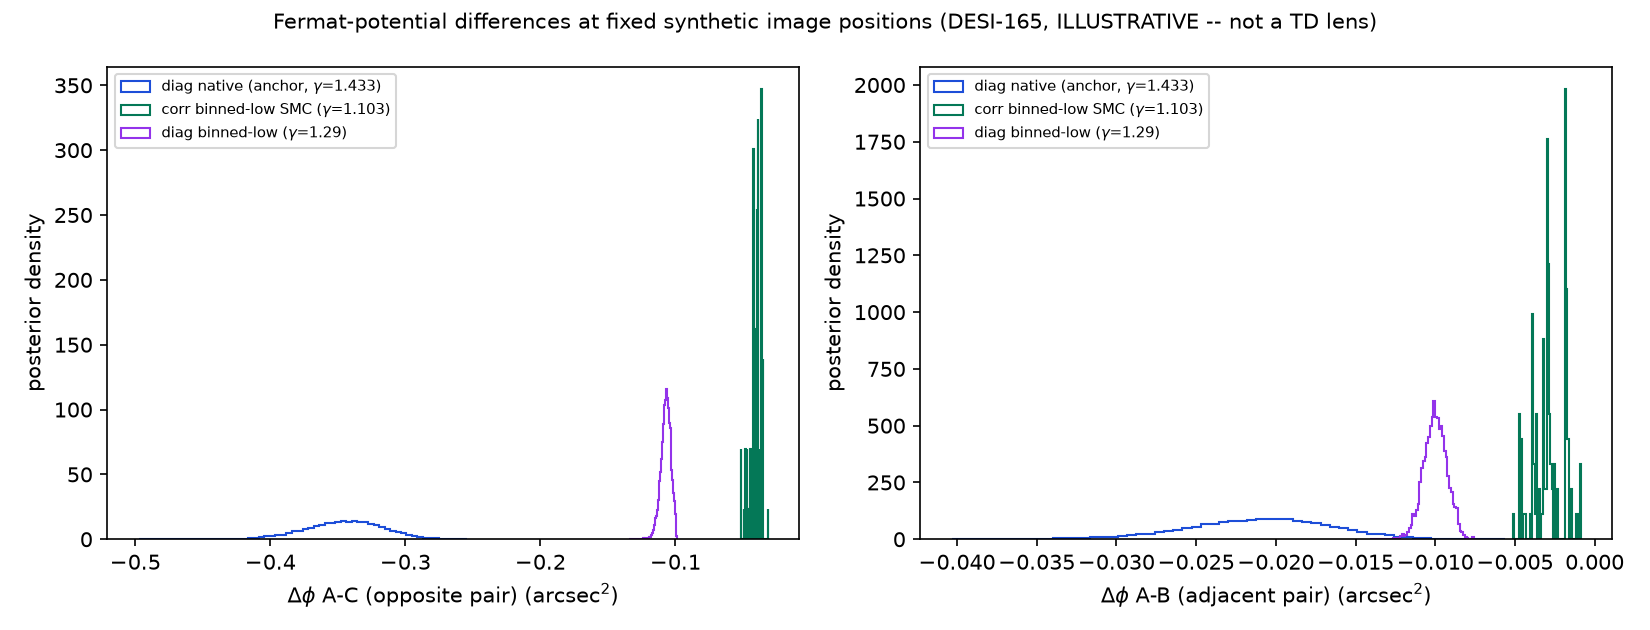
\includegraphics[width=0.88\textwidth]{../figs/fermat_dt_teaser.png}
\caption{Fermat-potential difference posteriors for an opposite and an
adjacent synthetic image pair under the three noise-model posteriors
(diagonal-native anchor, diagonal-binned-low, correlated-binned-low).
Illustrative only (see the triple disclaimer): the noise-model choice moves
$\Delta\phi$ by 61--88\% where $\sim$1\% is the TDCOSMO-relevant scale.
Source: \dfile{data/fermat\_dt\_teaser.json}.}
\label{fig:fermat}
\end{figure}
